%% ----------------------------------------------------------------
%% Thesis.tex -- main
%% ---------------------------------------------------------------- 

\documentclass[a4paper, 10pt, oneside]{memoir}
%% Use the option citeauthor to be able to use citet. The default cite will still work.
\usepackage[citeauthor]{basilea}

%% packages
\usepackage{amsmath}
\usepackage{tcolorbox}
\usepackage{multicol}
\usepackage{xskak} % chessboard

%% ----------------------------------------------------------------

\title				{Oxiflex - A Constraint Programming Solver for MiniZinc written in Rust}
\thesistype			{Bachelor's thesis}

\department 		    {Department of Mathematics and Computer Science}
\faculty			{Faculty Artificial Intelligence of the University of Basel}
\research		    {Research Group \\ https://ai.dmi.unibas.ch/}

\examiner    		{Examiner Prof. Dr. Malte Helmert}
\supervisor  		{Simon Dold}

\authors     		{Gianluca Klimmer}
\email				{gianluca.klimmer@stud.unibas.ch}
\immatriculnr		{2019-915-594}

\date				{Hand-In-Date}

% switch here for the german logo to logo-de
\ulogo				{Template/logo-en} 


%% ----------------------------------------------------------------
\begin{document}

\selectlanguage{english}

\thesisfront
\maketitle
\pagestyle{thesis}
%% ----------------------------------------------------------------
% % !TEX root = ../Thesis.tex
\chapter{Acknowledgments}
So Long, and Thanks for All the Fish. And the template.
%% ----------------------------------------------------------------
% !TEX root = ../Thesis.tex
\chapter{Abstract}
This thesis discusses the thesis template using some examples of the Turing Machine.
%% ----------------------------------------------------------------
\thesistoc
%% ----------------------------------------------------------------
%\thesisnomencl
%% ----------------------------------------------------------------
\thesismain

\chapter{Introduction}

test

\chapter{Constraint Satisfaction Problems} \label{chap:CSP}

\section{Constraint Satisfaction Problems}

Constraint Satisfaction Problems (CSP) \cite{csp:1987} are mathematical questions defined as a finite set of variables whose value must satisfy a number of constraints or limitations. When solely talking about the problem without the algorithmic finding of a solution, these are called Constraint Networks. CSPs are typical NP-complete combinatorial problems in the field of AI.

\begin{tcolorbox}[title=Example:]
	\begin{multicols}{2}
		\begin{equation*}
			\begin{aligned}
				w & = \{1, 2, 3, 4\} \\
				y & = \{1, 2, 3, 4\} \\
				x & = \{1, 2, 3\}    \\
				z & = \{1, 2, 3\}    \\
			\end{aligned}
		\end{equation*}

		\columnbreak

		\noindent
		\begin{equation*}
			\begin{aligned}
				\textbf{where:} \\
				w = 2 \cdot x   \\
				w < z           \\
				y > z           \\
			\end{aligned}
		\end{equation*}
	\end{multicols}
\end{tcolorbox}

We define variables $w$, $y$, $x$ and $z$. Variables $w$ and $y$ can both have one value from $\{1, 2, 3, 4\}$ and variables $x$ and $z$ can have a value from $\{1, 2, 3\}$. The constraints then restrict which values are valid from their respective domains. Here $w = 2 \cdot x$ restrict the value of $x$ to be double of $w$ for example. If there are no constraints for variables, the constraints are still there but they allow every assignment. These constraints are called trivial constraints and are usually omitted.

In this example we define constraints in a mathmatical notation. There are no formal restrictions on stating constraints neither by their complexity nor by the number of variables involved. To make it easier to reason about within this text, we model constraints as binary constraint sets. This is only for simplification. Constraints are then sets of valid value pairs for two specific variables. Instead of stating the desired relation between any variables, we list all valid value pair tuples in a set. Constraint $w < z$ then becomes $(R_{wz} = \{(1, 2), (1, 3), (2, 3)\}$ which contains all possible value pairs for the two varaibles $w$ and $z$.

We define Constraint Networks formally:

\begin{tcolorbox}
	A (binary) constraint network is a 3-tuple $C = <V, \text{dom}, (R_{uv})>$ such that:
	\begin{itemize}
		\item $V$ is a non-empty and finite set of variables,
		\item dom is a function that assigns a non-empty and finite domain to each variable $v \in V$, and
		\item $(R_{uv})_{u,v \in V, u \neq v}$ is a family of binary relations (constraints) over $V$ where for all $u \neq v: R_{uv} \subseteq \text{dom}(u) \times \text{dom}(v)$
	\end{itemize}
\end{tcolorbox}

And we define our example formally:

\begin{tcolorbox}
	$C = \langle V, \text{dom}, (R_{uv})\rangle$ with
	\begin{itemize}
		\item variables: \\
		      $V = \{w, x, y, z\}$
		\item domains: \\
		      $\text{dom}(w) = \text{dom}(y) = \{1, 2, 3, 4\}$ \\
		      $\text{dom}(x) = \text{dom}(z) = \{1, 2, 3\}$
		\item constraints: \\
		      $R_{wx} = \{(2, 1), (4, 2)\}$ \\
		      $R_{wz} = \{(1, 2), (1, 3), (2, 3)\}$ \\
		      $R_{yz} = \{(2, 1), (3, 1), (3, 2), (4, 1), (4, 2), (4, 3)\}$ \\
	\end{itemize}
\end{tcolorbox}

The goal in CSP is then to find a Assignment that satisfies all constraints. For this simple example a possible assignment would be $(w \mapsto 2), (x \mapsto 1), (y \mapsto 4), (z \mapsto 3)$.

\section{MiniZinc}

MiniZinc~\cite{minizinc:2007} is a free and open-source constraint modeling language developed at and by Monash University in Australia. It allows us to express Constraint Satisfaction Problems in a mathmatical notation-like way.

\begin{tcolorbox}[title=MiniZinc example]
	var 1..4: w; \\
	var 1..4: y; \\
	var 1..3: x; \\
	var 1..3: z; \\

	constraint w = 2 $\times$ x; \\
	constraint w $<$ z; \\
	constraint y $>$ z; \\

	solve satisfy;
\end{tcolorbox}

MiniZinc is only the language to express a problem domain. Once a problem domain is specified in MiniZinc we can give the problem to multiple solvers to solve them. In this way we can compare the performance of various solvers on the same problem domain. MiniZinc Domain files have the file extension \verb|.mzn|.

MiniZinc also provides a way to parametrize a problem domain. This is a great way to scale a problem space up and see how increasing the problem size affects the solving speed. A great example for this is the Queens Problem (See Section~\ref{sec:queens}). We define the Queens Problem domain once and can then run specific problem instances for different $n$. This makes it really easy to compare the solving speed for the queens problem when $n = 8$, $n = 16$ or $n = 32$. Files where we specify parameters for MiniZinc files are called data files and have the extension \verb|.dzn|. We can than combine \verb|.mzn| files with \verb|.dzn| files to created FlatZinc files.

\subsection{FlatZinc}

FlatZinc is a simpler problem specification language provided by the MiniZinc package. It is designed to be used by solvers directly. MiniZinc files are translated to FlatZinc files in a pre-solving step. FlatZinc files have the file extension \verb|.fzn|.

Translating from MiniZinc to FlatZinc maps more advanced instructions from MiniZinc to primitives supported in FlatZinc. An analogy to this translation is compiling a C program to Assembly where MiniZinc is C and FlatZinc is Assembly. FlatZinc therefore requires solvers to support a set of standard contraints called FlatZinc builtins. Builtins need to be implemented to be a fully compatible FlatZinc solver. See the following for an FlatZinc translation using our simple example.

\begin{tcolorbox}[title=Simple example translated to FlatZinc (Simplified)]
	array [1..2] of int: x\_introduced\_2\_ = [1,-2]; \\
	array [1..2] of int: x\_introduced\_3\_ = [1,-1]; \\
	array [1..2] of int: x\_introduced\_4\_ = [-1,1]; \\
	var 2..4: w:: output\_var; \\
	var 1..4: y:: output\_var; \\
	var 1..3: x:: output\_var; \\
	var 1..3: z:: output\_var; \\
	constraint int\_lin\_eq(x\_introduced\_2\_,[w,x],0); \\
	constraint int\_lin\_le(x\_introduced\_3\_,[w,z],-1); \\
	constraint int\_lin\_le(x\_introduced\_4\_,[y,z],-1); \\
	solve  satisfy;
\end{tcolorbox}

The translation of the variable declations is straight forward. For the constraints, MiniZinc translated all constraints into FlatZinc builtin constraints. For our simple example MiniZinc used two builtins: \verb|int_lin_eq| and \verb|int_lin_le|. See the lines that start with \verb|constraint|. We will look at \verb|int_lin_eq| further to see how FlatZinc builtins work. The following is the signature of the builtin \verb|int_lin_eq| that was used for the constraint $w = 2 \cdot x$.

\begin{tcolorbox}[title=int\_lin\_eq builtin signature]
	predicate int\_lin\_eq(array [int] of int: as,\\
	array [int] of var int: bs,\\
	int: c)
\end{tcolorbox}

Note that the builtin \verb|int_lin_eq| expects 3 parameters. The first \verb|as| is an array of \verb|int| constants. This is what the example FlatZinc translation named \verb|x_introduced_2|. This array is called a parameter, because it has concrete values assigned to it. Here \verb|x_introduced_2| has the value \verb|[1,-2]| assigned. The second parameter \verb|bs| is an array of \verb|int| variables, that is an array of variables that we want to solve for. Here the variables $w$ and $x$ are passed in also as an array \verb|[w,x]|. The third parameter \verb|c| is also a parameter because it is also a constant value that needs to be passed. Here the value for \verb|c| is $0$.

Every FlatZinc builtin also has a description for when the constraint is valid or violated respectively. For \verb|int_lin_eq| the description is as follows.

\begin{tcolorbox}[title=int\_lin\_eq builtin constraint]
	\begin{equation}
		c = \sum_{i} \text{as}[i] \cdot \text{bs}[i]
	\end{equation}
\end{tcolorbox}

For this builtin MiniZinc translated our constraint into a linear combination. With our example we can fill in the passed parameters to the constraint and we get $0 = w - 2x$ which can be rearranged to $w = 2 \cdot x$.

Note that FlatZinc created these parameter arrays by itself. The \verb|x| within \verb|x_introduced_2_| is not the same as our variable $x$ that we defined within MiniZinc.

Also note that for the translation MiniZinc already does some basic level of inference. The FlatZinc variable $w$ can only have values between $2$ and $4$ in the translated FlatZinc. Whereas in the MiniZinc version we defined $w$ with the domain $\{1, 2, 3, 4\}$. This means MiniZinc infers that $w$ can not be value $1$ and removes it from its domain declaration. Due to the constraint $w = 2 \times x$, the variable $w$ has to be double of $x$ and $x$ must have at least value $1$. Therefore excluding $1$ as possible value for $w$.

\section{Queens Problem} \label{sec:queens}

Also called the Eight Queens Puzzle, the Queens Problem is an example of a classic constraint satisfaction problem that involves placing eight queens on an 8x8 chessboard in such a way that no two queens threaten each other. That is, no two queens can share the same row, column, or diagonal. See the following for an example solution to the 8-Queens Problem.

\newchessgame
\chessboard[setfen=1Q6/3Q4/5Q2/7Q/2Q5/Q7/6Q1/4Q3 w - - 0 1, showmover=false] \\

The Eigth Queens Puzzle is really good suited as an example problem domain for constraint satisfaction problems because it is easy to understand and can also easily be scaled up to increase complexity for a solver. By generalizing the problem from a fixed $8 \times 8$ grid size to an $n \times n$ grid with $n$ queens, the problem remains the same in principle, but gets way harder to solve. See the following example of the queens problem modeled in MinZinc \cite{minizinc_queens:2006}.

\begin{tcolorbox}[title=MiniZinc Model for N-Queens Problem]
	int: n; \\

	array [1..n] of var 1..n: q; \\

	predicate \\
	noattack(int: i, int: j, var int: qi, var int: qj) = \\
	qi     != qj     /\textbackslash \\
	qi + i != qj + j /\textbackslash \\
	qi - i != qj - j; \\

	constraint \\
	forall (i in 1..n, j in i+1..n) ( \\
	noattack(i, j, q[i], q[j]) \\
	); \\

	solve satisfy;
\end{tcolorbox}

This MiniZinc model defines an array of variables $q$ where each index corresponds to a column on the chessboard and the value at each index represents the row position of the queen in that column. The constraints ensure that no two queens are on the same row, column or diagonal.


\chapter{Solving Constraint Satisfaction Problems}

Constraints satisfaction problems on finite domains are typically solved using a form of search. We search for a solution to the constraint network by trying out all possible values until a solution is found. That is, a valid assignment of all variables with a value of their respective domain satisfing all constraints within the constraint network.

\section{Naive Backtracking}

Backtracking is a technique used to search a problem space for potential solutions \cite{backtracking:1975}. It systematically organizes the search process by attempting to extend a partial solution step-by-step. If an extension of the current partial solution proves unfeasible at any stage, the algorithm "backtracks" to a previous, shorter partial solution and tries a different path. This method is particularly useful in solving constraint satisfaction problems, as demonstrated by the algorithm called NaiveBacktracking.

\begin{tcolorbox}[title=function NaiveBacktracking)]
	$\langle V, \text{dom}, (R_{uv})\rangle := C$ \\
	\textbf{if} $\alpha$ is inconsistent with $C$: \\
	\textbf{return inconsistent} \\

	\textbf{if} $\alpha$ is a total assignment: \\
	\textbf{return $\alpha$} \\

	select some variable $v$ for which $\alpha$ is not defined \\
	\textbf{for each} $d \in$ dom($v$) in some order: \\
	$\alpha' := \alpha \cup \{v \mapsto d\}$ \\
	$\alpha'' := $ NaiveBacktracking($C$, $\alpha'$) \\
	\textbf{if} $\alpha'' \neq$ \textbf{inconsistent}: \\
	\textbf{return} $\alpha''$ \\

	\textbf{return inconsistent}
\end{tcolorbox}

Input: constraint network $C$ and partial assignment $\alpha$ for $C$. On first invocation of NaiveBacktracking we pass an empty assignment $\alpha = \emptyset$. \\
Result: Total assignment (solution) of $C$ or \textbf{inconsistent}.

This algorithm corresponds to Depth First Search (DFS). It assigns values to variables from their domains to form a partial assignment. This process continues until either all variables are assigned and a solution is found, or a constraint is violated. If a constraint is violated, the algorithm backtracks and tries a different value from the domain until a solution is found. If all possible assignments violate constraints, there is no solution. Finding a total assignment, that is an partial assignment that gives each variable a valid value from its domain, is finding a solution.

Backtracking is far from the best way to solve CSPs.

\subsection{Variable Ordering}

Backtracking in general does not specify in which order the search is done. For constraint satisfaction problems we want to assign critical variables early. Critical variables are variables that thighten the search space the most by their assignment. This can be done in multiple ways:
\begin{itemize}
	\item \textbf{static order} \\
	      Fixed order defined prior to search
	\item \textbf{dynamic order} \\
	      Order depends on current search state and is calculated after each assignment
\end{itemize}

\section{Inference} \label{inference}

Inference allows us to modify our constraint network by thightening the constraint network. Thightening works by excluding values from domains of variables that we know are not possible. For example in the Queens Problem (See \ref{sec:queens}) if we place a Queen on $d4$, we can exclude the value $4$ from all other files (chess term for column). We can also exclude all diagonally positioned squares like $a1$, $b2$, $c3$ and so forth. See \ref{chess:queeninference} for reference. Note that we do not need to do anything with the file the queen is on because we modeled the file to be a variable to solve for and a variable can only how one value anyways.

\newchessgame
\chessboard[
	setfen=8/8/8/8/3Q4/8/8/8 w - - 0 1,
	color=blue!50,
	pgfstyle=color,
	markfields={a7,b6,c5,a4,b4,c4,a1,b2,c3,e5,f6,g7,h8,e4,f4,g4,h4,e3,f2,g1},
	showmover=false
]
\label{chess:queeninference}

By removing impossible values from the remaining domains, we can thighten the resulting constraint network and have a smaller search space. We adjust our NaiveBacktracking approach by applying inference after each assignment of an variable. See the following for the NaiveBacktracking algorithm.

\begin{tcolorbox}[title={function BacktrackingWithInference($C, \alpha$)}]
	$\langle V, \text{dom}, (R_{uv})\rangle := C$ \\
	\textbf{if} $\alpha$ is inconsistent with $C$: \\
	\textbf{return inconsistent} \\

	\textbf{if} $\alpha$ is a total assignment: \\
	\textbf{return $\alpha$} \\

	$C' := \langle V, \text{dom}',(R'_{uv})\rangle :=$ copy of $C$ \\
	apply inference to $C'$ \\
	if dom$'(v) \neq \emptyset$ for all variables $v$: \\

	select some variable $v$ for which $\alpha$ is not defined \\
	\textbf{for each} $d \in$ copy of dom$'(v)$ in some order: \\
	$\alpha' := \alpha \cup \{v \mapsto d\}$ \\
	dom$'(v) := \{d\}$ \\
	$\alpha'' := $ BacktrackingWithInference($C'$, $\alpha'$) \\
	\textbf{if} $\alpha'' \neq$ \textbf{inconsistent}: \\
	\textbf{return} $\alpha''$ \\

	\textbf{return inconsistent}
\end{tcolorbox}

Note that we now have to copy the constraint network after each assignment which can introduce significant overhead for simple problems. The coping is needed because we still have to backtrack if we find an inconsistent assignment. When backtracking we have to restore the domain for each variable again because it is possible that the domain had values that are possible again after backtracking.

\subsection{Forward Checking}

We start with a simple inference method called Forward Checking \cite{forward_checking:1980}. See the following algorithm.

\begin{tcolorbox}[title={function ForwardChecking($C, \alpha$)}]
	for each $v \in $ unassigned variables in $\alpha$:

	for each constraint:

	\textbf{if} any $d \in$ dom($v$) in conflict:
	dom($v$) = dom($v$) $\setminus d$
\end{tcolorbox}

Forward checking is basically looking ahead in the future to see which values can be excluded from search after an assignment. By looking ahead we can ommit the backtracking part that would result by finding a dead end. We check each value for each variable with the new assignment and remove all values that are not possible anymore from their respective domain.

\subsection{Arc Consistency}

Arc consistency excludes all impossible values from all domains of all variables in a given constraint network. Originally developed for vision problems \cite{original_arc:1988} arc consistency is the generalization of forward checking. Forward checking enforces arc consistency for all variables with respect to the just assigned variable. Arc consistency does this for all variables. This makes forward checking a special case of arc consistency. See the following for formal definition.

\begin{tcolorbox}[title=Definition: Arc Consistent]
	Let $C = \langle V$, dom, $(R_{uv})\rangle$ be a constraint network.
	\begin{itemize}
		\item The variable $v \in V$ is arc consistent with respect to another variable $v'\in V$, if for every value $d \in$ dom($v$) there exists a value $d' \in$ dom($v'$) with $\langle d, d' \rangle \in R_{vv'}$.
		\item The constraint network $C$ is arc consistent, if every variable $v \in V$ is arc consistent with respect to every other variable $v' \in V$.
	\end{itemize}
\end{tcolorbox}

Note that for a variable pair the definition is not symmetrical. That means if $v$ is arc consistent with respect to $v'$, $v'$ does not have to be arc consistent with respect to $v'$.

\subsubsection{Enforcing Arc Consistency}

There are multiple algorithms to enforce arc consistency \cite{arc_studied:1977} \cite{arc_again:1994}. The simplest is called AC-1. It works by making use of a function called revise. The following function revise ensures arc consistency in one direction between two variables.

\begin{tcolorbox}[title={\textbf{function} revise($C,v,v'$):}]
	$\langle V,$ dom, $(R_{uv})\rangle := C$ \\
	\textbf{for each} $d \in$ dom($v$): \\
	\textbf{if} there is no $d' \in$ dom($v'$) with $\langle d, d' \rangle \in R_{vv'}$: \\
	\textbf{remove} $d$ from dom($v$)
\end{tcolorbox}

The following algorithm AC-1 goes over each constraint and applies revise in both directions to each variable pair for each constraint until there was no change within its iteration of using revise.

\begin{tcolorbox}[title={\textbf{function} AC-1($C$):}]
	$\langle V,$ dom, $(R_{uv})\rangle := C$ \\
	\textbf{repeat} \\
	\textbf{for each} nontrivial constraint $R_{uv}$: \\
	revise($C, u, v$) \\
	revise($C, v, u$) \\
	\textbf{until} no domain has changed in this iteration
\end{tcolorbox}

Building on AC-1, AC-3 tries to save redundant checks made by AC-1. Instead of just going over all constraints over and over, we go at least over all constraint once and revise variable pairs again only if needed. In AC-3 this can be achived by using a queue. See the following for reference.

\begin{tcolorbox}[title={\textbf{function} AC-3($C$):}]
	$\langle V,$ dom, $(R_{uv})\rangle := C$ \\
	queue $:= \emptyset$ \\
	\textbf{for each} nontrivial constraint $R_{uv}$: \\
	insert $\langle u, v \rangle$ into \textit{queue} \\
	insert $\langle u, v \rangle$ into \textit{queue} \\

	\textbf{while} \textit{queue} $\neq \emptyset$: \\
	remove an arbitrary element $\langle u, v \rangle$ from \textit{queue} \\
	revise($C, u, v$) \\
	\textbf{if} dom($u$) changed in the call to revise: \\
	\textbf{for each} $w \in V \setminus \{u,v\}$ where $R_{wu}$ is nontrivial: \\
	insert $\langle w, u \rangle$ into \textit{queue}
\end{tcolorbox}


\chapter{Oxiflex}

As part of this thesis we present \textbf{oxiflex}, a minimal constraint satisfaction problem solver from scratch for MiniZinc written in Rust. Oxiflex is a FlatZinc solver that can be used as an backend to MiniZinc. This means oxiflex minimally supports the requirements for a solver to take advantage of the MiniZinc toolchain. The goal is to have a minimal solver and be able measure the impact of various improvements like forward checking on constraint satisfaction problem solvers.

Oxiflex is open-source and licensed under the MIT license. It is available at Github \url{https://github.com/glklimmer/oxiflex}.

\section{Rust}

Rust \cite{rust:2014} is a general purpose systems programming language focused on safety and performance. It achieves these goals without using a garbage collector by ensuring memory safety through a system of ownership with strict compile-time checks enforced by the borrow checker. This makes Rust particularly well-suited for creating performance-critical applications like CSP solvers where control over resources is crucial. This makes Rust an ideal choice for developing oxiflex.

\section{Dependecies}

This work depends on previous work by others. This section highlights the components used by oxiflex.

\subsection{flatzinc} \label{flatzinc}

The library flatzinc~\cite{flatzinc:2020} is a FlatZinc parser for Rust. It parses the FlatZinc format into Rust structures and variables.

\subsection{structopt}

The library structopt~\cite{structopt:2020} is utilized to parse command-line arguments in oxiflex. This library simplifies setting up custom commands and options for oxiflex.

\subsection{hyperfine}

The librabry hyperfine~\cite{hyperfine:2023} is a command-line benchmarking tool. We use hyperfine to measure and compare the performance of different solver strategies and optimizations.

\section{Architecture}

There are three main parts of oxiflex.

\begin{itemize}
	\item parser
	\item model
	\item solver
\end{itemize}

\subsection{parser}

Using the library flatzinc \ref{flatzinc} oxiflex reads an FlatZinc \verb|.fzn| file and collects all parts needed to then construct a constraint satisfaction network. These include a list for parameters, variables and constraints. In order to also output the solution after solving the problem, MiniZinc makes use of annonations on FlatZinc elements. Variables that are needed for the output are annotated as \verb|output_var|. There are two possible output annotations in FlatZinc: \verb|output_var| and \verb|output_array|.

\subsection{model} \label{model}

After parsing the FlatZinc file into Rust structures that can be used directly, oxiflex starts to build useful structures  to solve any given problem. This is where oxiflex creates a model containing variables with their respectice domains and constraints. Models use HashMaps to keep track of its variables and their respective domains. This allows for constant access time to domains to either read or modify them after inference (\ref{inference}) for example. Constraints are saved by the model as a list (In rust this is a pointer, capacity, length triplet). Usually when checking if constraints are violated we either want all constraints or all constraints related to a variable. For this reason an additional HashMap is created called \verb|constraint_index|, that uses variable ids as key and points to a list of constraints on the heap. In rust this can be done by using reference counting. This results in two ways to access constraints. One that is just a list to iterate over all constraints and one where a hashmap is used to get all constraints involved by a specific variable.

Variables all have an id. All variable ids are strings. Oxiflex also uses reference counting to store variable ids. As it is often also needed to pass variable ids around, we can mitigate the cost of calling \verb|clone| on variable ids by using reference counting. Instead of actually cloning variable ids, we just pass a pointer to the variable id needed. With reference counting we can ensure the actual memory for the variable id is freed after all pointers to it have been deleted.

\subsection{Limitations}

There are some limitations due to time constraints that currently limit oxiflex as a universal MiniZinc solver. \\

Not all FlatZinc builtins are supported. The idea is to implement just the needed builtins for any given insteresting problem domain.
% Maybe add roadmap?

% TODO: Only ints are available

% TODO: Only solving, no optimization

\section{Solver}

The solver is the core part of oxiflex. By allowing control over what optimization is turned on or off we can measure the impact of each optimization individually. As discussed in Chapter \ref{solving_csp}: \nameref{solving_csp}, there are various optimizations for solving CSPs. See the following diagram to see all optimizations implemented in oxiflex. \\

\begin{tikzpicture}[node distance=2cm and 3cm, auto]
	% Styles
	\tikzset{
		abstraction/.style={draw, rectangle, fill=red!20, text width=10em, text centered, minimum height=2.5em},
		file/.style={draw, rectangle, fill=blue!20, text width=10em, text centered, minimum height=2.5em},
		method/.style={draw, ellipse, fill=green!20, text width=5em, text centered, minimum height=3em},
		line/.style={draw, -Latex}
	}

	% Nodes
	\node[abstraction] (solver) {Solver};

	\node[file, below left of=solver, node distance=3cm] (naiveBT) {naive\_backtracking.rs};
	\node[file, below right of=solver, node distance=3cm, xshift=2cm] (inferenceSolver) {inference.rs};

	\node[method, below=1cm of naiveBT, xshift=0.5cm] (varOrder1) {Variable Ordering};
	\node[method, below=1cm of inferenceSolver, xshift=-2cm] (forwardCheck) {Forward Checking};
	\node[method, below=1cm of inferenceSolver, xshift=1cm] (arc1) {AC-1};
	\node[method, right=0cm of arc1, yshift=0.7cm] (arc3) {AC-3};

	% Lines
	\path[line] (solver) -- (naiveBT);
	\path[line] (solver) -- (inferenceSolver);
	\path[line] (naiveBT) -- (varOrder1);
	\path[line] (inferenceSolver) -- (varOrder1);
	\path[line] (inferenceSolver) -- (forwardCheck);
	\path[line] (inferenceSolver) -- (arc1);
	\path[line] (inferenceSolver) -- (arc3);

\end{tikzpicture} \\

By default each optimization in oxiflex is turned on. By passing flags named after each optimization we can disable the respective optimization. The help menu can be printed using \verb|oxiflex --help| from the console.

\begin{verbatim}
FLAGS:
    -f, --forward-checking
    Use forward checking as inference

    -n, --naive-backtracking
    Use naive backtracking, e.g. no forward_checking

    -r, --random-variable-order
    Use random order for variable ordering.

    -a, --arc-consistency <arc-consistency>
    Specify arc consistency version [default: 3]
\end{verbatim}

\subsection{Value Ordering}

Oxiflex is able to use dynamic ordering of variables during search based on the number of constraints. Enabled by default, oxiflex orders variables from most constraints involvment to least for assignment. This fail early approach to ordering can be used both for NaiveBacktracking and Inference based algorithms.

\subsection{Forward Checking}

Forward checking in oxiflex works by removing impossible values inplace of their domains. Doing forward checking in an immutable manner, that is copying each domain, making changes to it and then saving it back to the model, is was more inefficient.

\subsection{Arc Consistency}

Both AC-1 and AC-3 use the function \verb|revise| which ensures arc consistency in one direction for two variables. The main computational work happens within this function. AC-1 and AC-3 only arrange the calls to \verb|revise| differently. Within \verb|revise| the \verb|constraint_index| (See \ref{model}: \nameref{model}) is used to get all constraints that are involved with a specific variable.
% TODO: write stuff


\chapter{Results}

Results, Graphs and stuff.

\begin{figure}[ht]
	\centering
	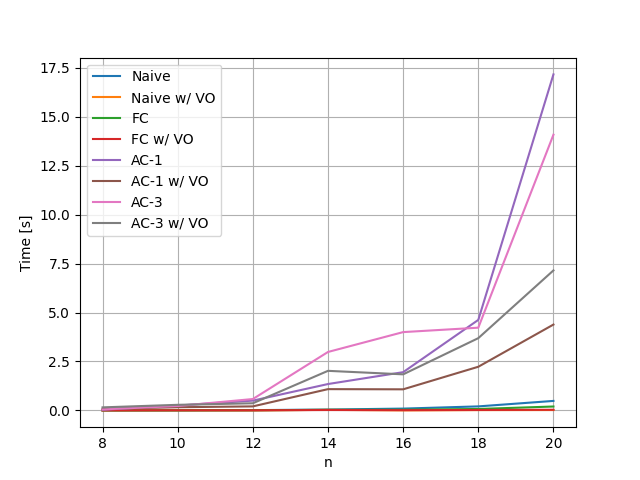
\includegraphics[width=0.8\textwidth]{./Problems/queens/plots/time.png}
	\caption{a nice plot}
	\label{fig:queens:time}
\end{figure}


\begin{figure}[ht]
	\centering
	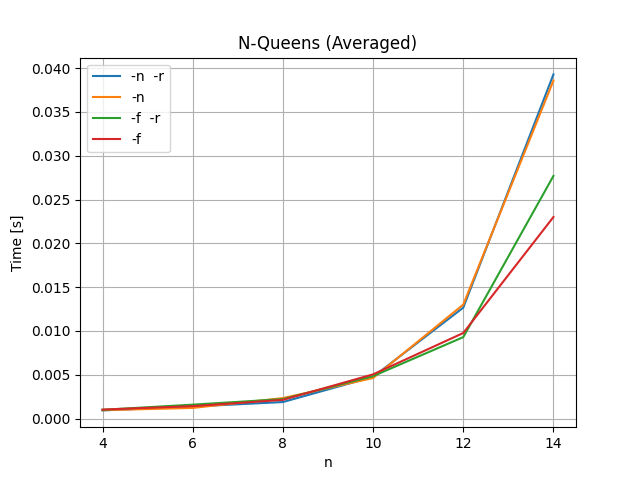
\includegraphics[width=0.8\textwidth]{./Problems/queens/plots/time_no_arc.png}
	\caption{a nice plot}
	\label{fig:queens:time_no_arc}
\end{figure}



\begin{figure}[ht]
	\centering
	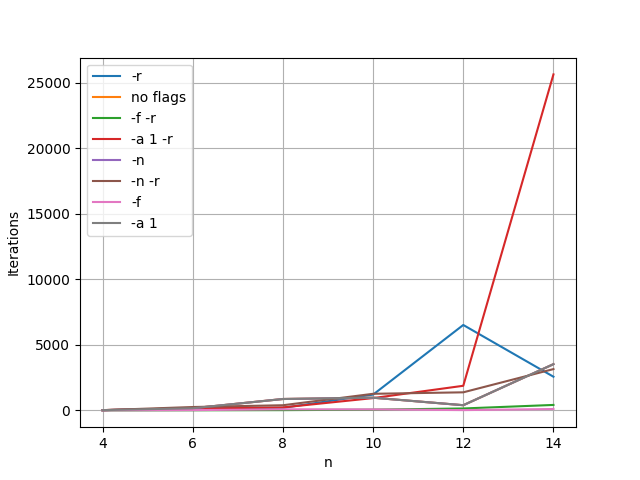
\includegraphics[width=0.8\textwidth]{./Problems/queens/plots/iterations.png}
	\caption{a nice plot}
	\label{fig:queens:iterations}
\end{figure}



\begin{figure}[ht]
	\centering
	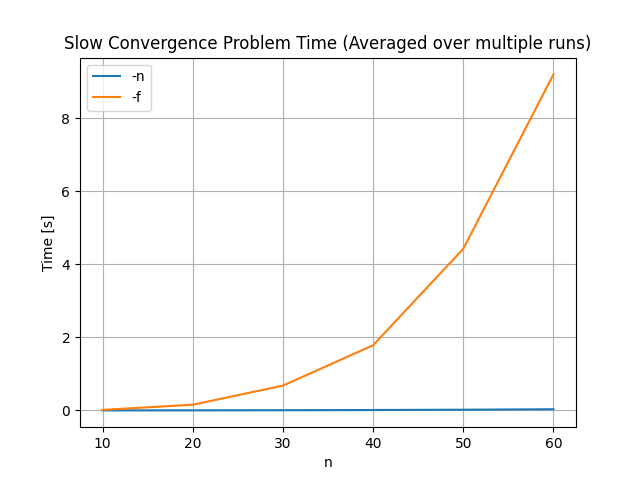
\includegraphics[width=0.8\textwidth]{./Problems/slow_convergence/plots/time.png}
	\caption{a nice plot}
	\label{fig:slow:time}
\end{figure}


\begin{figure}[ht]
	\centering
	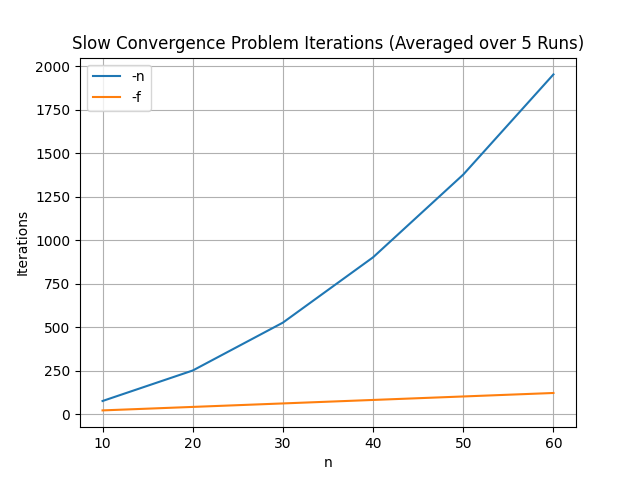
\includegraphics[width=0.8\textwidth]{./Problems/slow_convergence/plots/iterations.png}
	\caption{a nice plot}
	\label{fig:slow:iterations}
\end{figure}


\begin{figure}[ht]
	\centering
	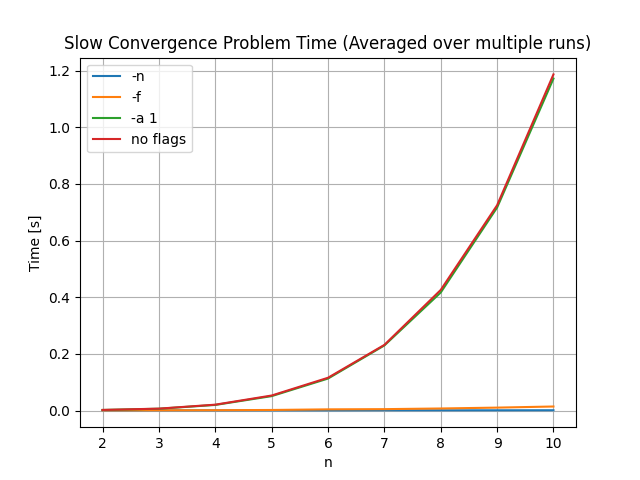
\includegraphics[width=0.8\textwidth]{./Problems/slow_convergence/plots/time_small.png}
	\caption{a nice plot}
	\label{fig:slow:time_small}
\end{figure}

\begin{figure}[ht]
	\centering
	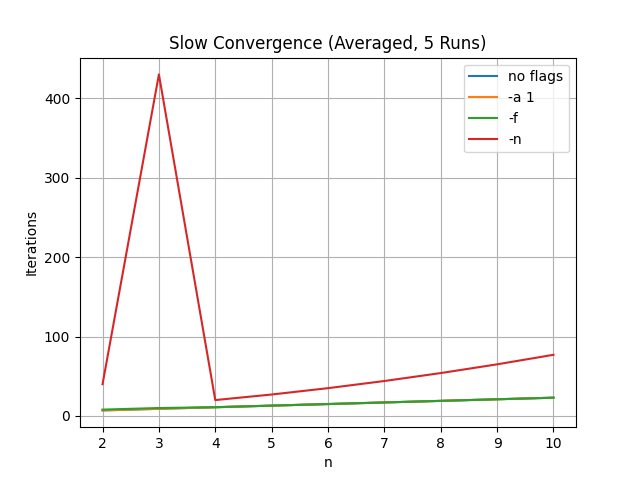
\includegraphics[width=0.8\textwidth]{./Problems/slow_convergence/plots/iterations_small.png}
	\caption{a nice plot}
	\label{fig:slow:iterations_small}
\end{figure}


\chapter{Conclusion} \label{chap:conclusion}

\section{Discussion}

The goal of this thesis was to create a Constraint Satisfaction Problem Solver from scratch. Within this thesis we developed Oxiflex, a CSP solver from scratch written in Rust. The solver supports the CSP modeling language MiniZinc through implementing a subset of FlatZinc builtin constraints.

We started by discussing what CSPs exactly are and by writing them down formally and in the MiniZinc language. Further we especially looked at the Queens Problem as an easy to understand CSP. Next we discussed possible techniques to solve CSPs using a method called backtracking. We started by using a naive form of the algorithm and improved it further. The first improvement discussed was variable ordering with an fail early approach. That means that we choose variables to assign first, that have the most constraints. We then improved on the backtracking algorithm by adding inference. Starting with forward checking, introducing arc consistency and finally discussing AC-1 and AC-3, arc consistency enforcing algorithms.

Furthermore we gave insights into how Oxiflex works and what data structures are used to solve CSPs within Oxiflex. We discussed how the improvements like forward checking and arc consistency within Oxiflex work and what structures are in place to support them.

Finally we measured how each improvement effected both Time and number of Iterations needed for solving the N-Queens and the Slow Convergence Problems in Oxiflex. It is great to see the trade off between search and inference. As we saw in~\cref{fig:slow:sidebyside} that showed the inverse correlation between Time and number of Iterations. Although it took longer to solve, inference did reduce the number of iterations significantly. It is interesting to observe the effect that variable ordering has for the slow convergence problem. In fact it made it even possible to solve the problem at all in under 300 seconds. It can be useful to measure other things than time (like iterations) to gather insights like these.

Therefore the main takeaway for this thesis is that data structures matter. Although an algorithm performs better in theory, the right data structures have to be used to make it really go faster. Using HashMaps to hold all the data might not be the best approach if performance is the main criteria of a program. This also underlines that just using a fast programming language is not sufficient to make a program go fast.


%% ----------------------------------------------------------------
\thesisappendix
\thesisbib
\begin{appendices}
	
\chapter{Appendix}
\end{appendices}
%% ----------------------------------------------------------------
\thesisback
\iflanguage{english}
{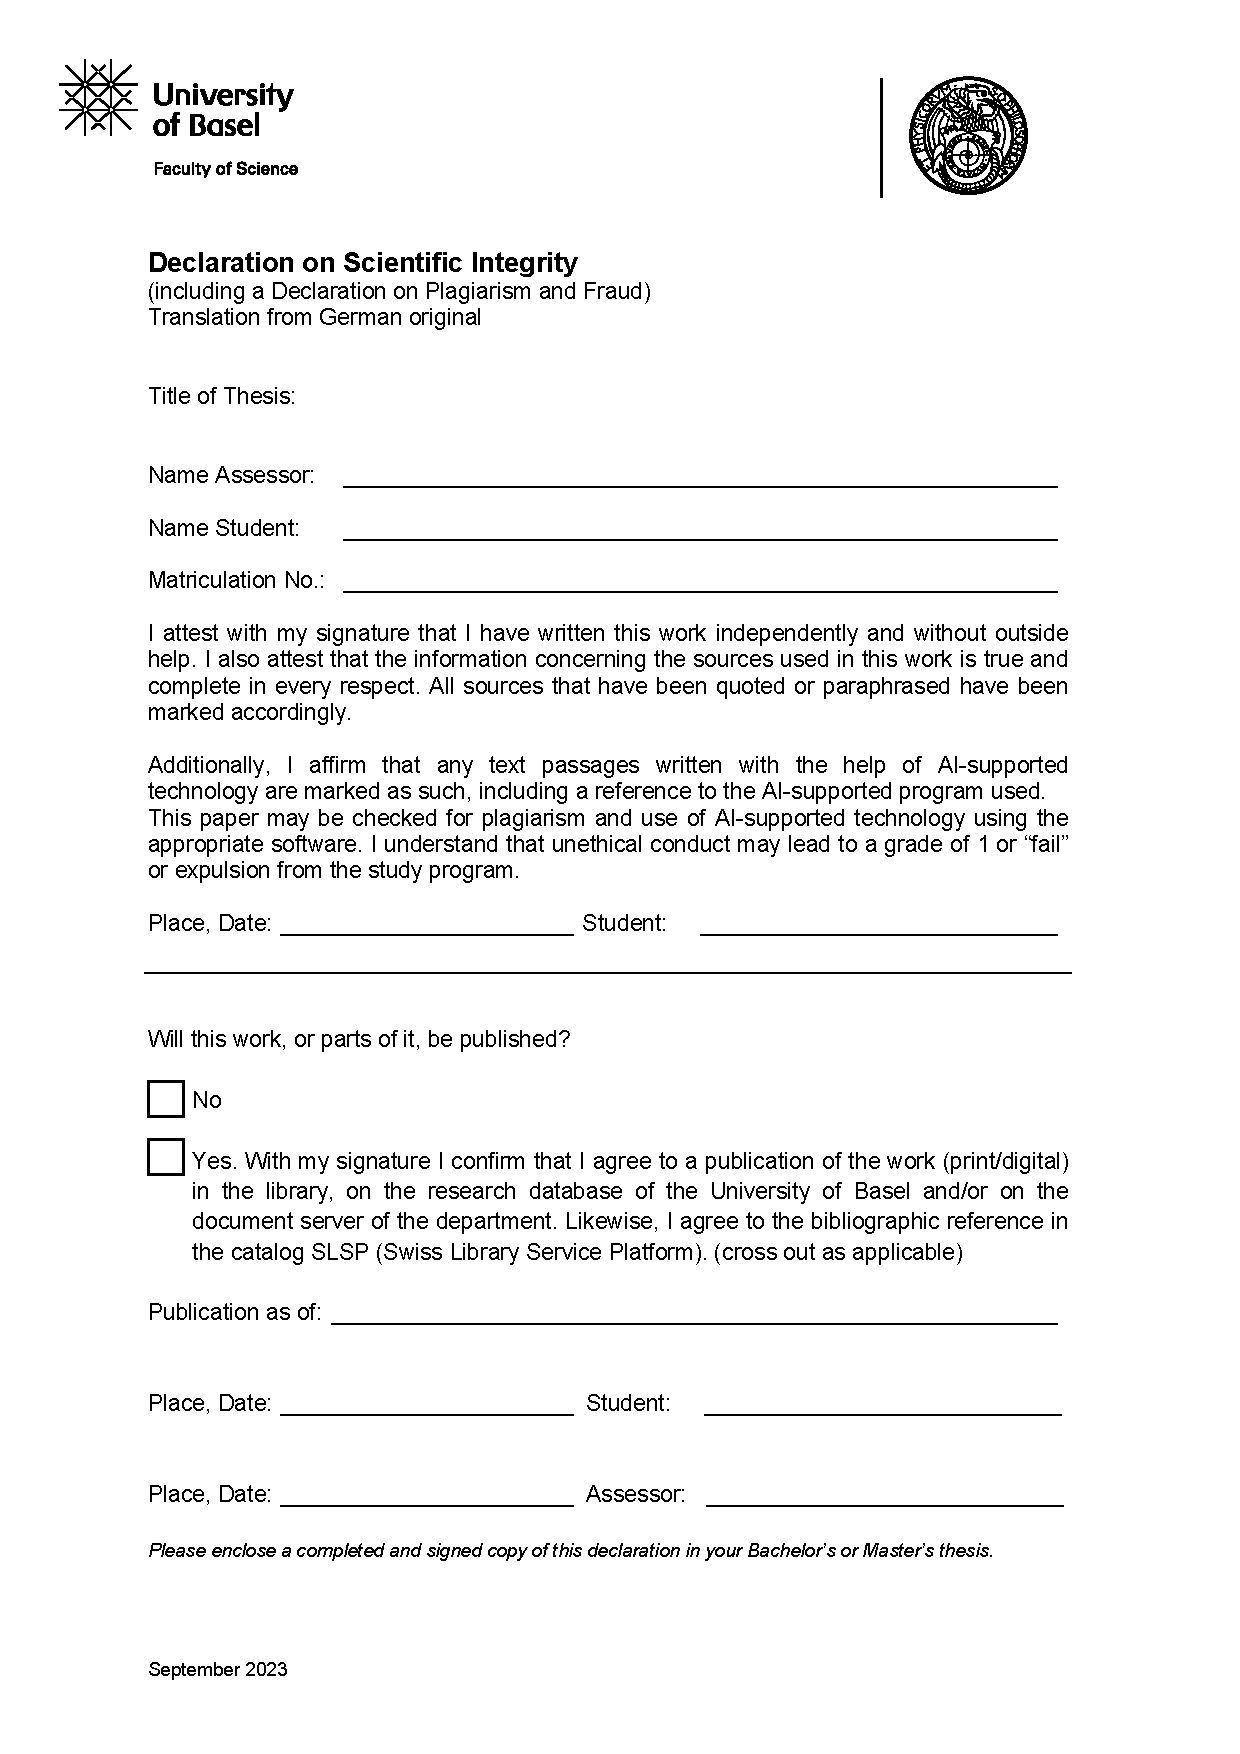
\includepdf{./Back/wissensch_Redlichkeit_E_09-2023.pdf}}
{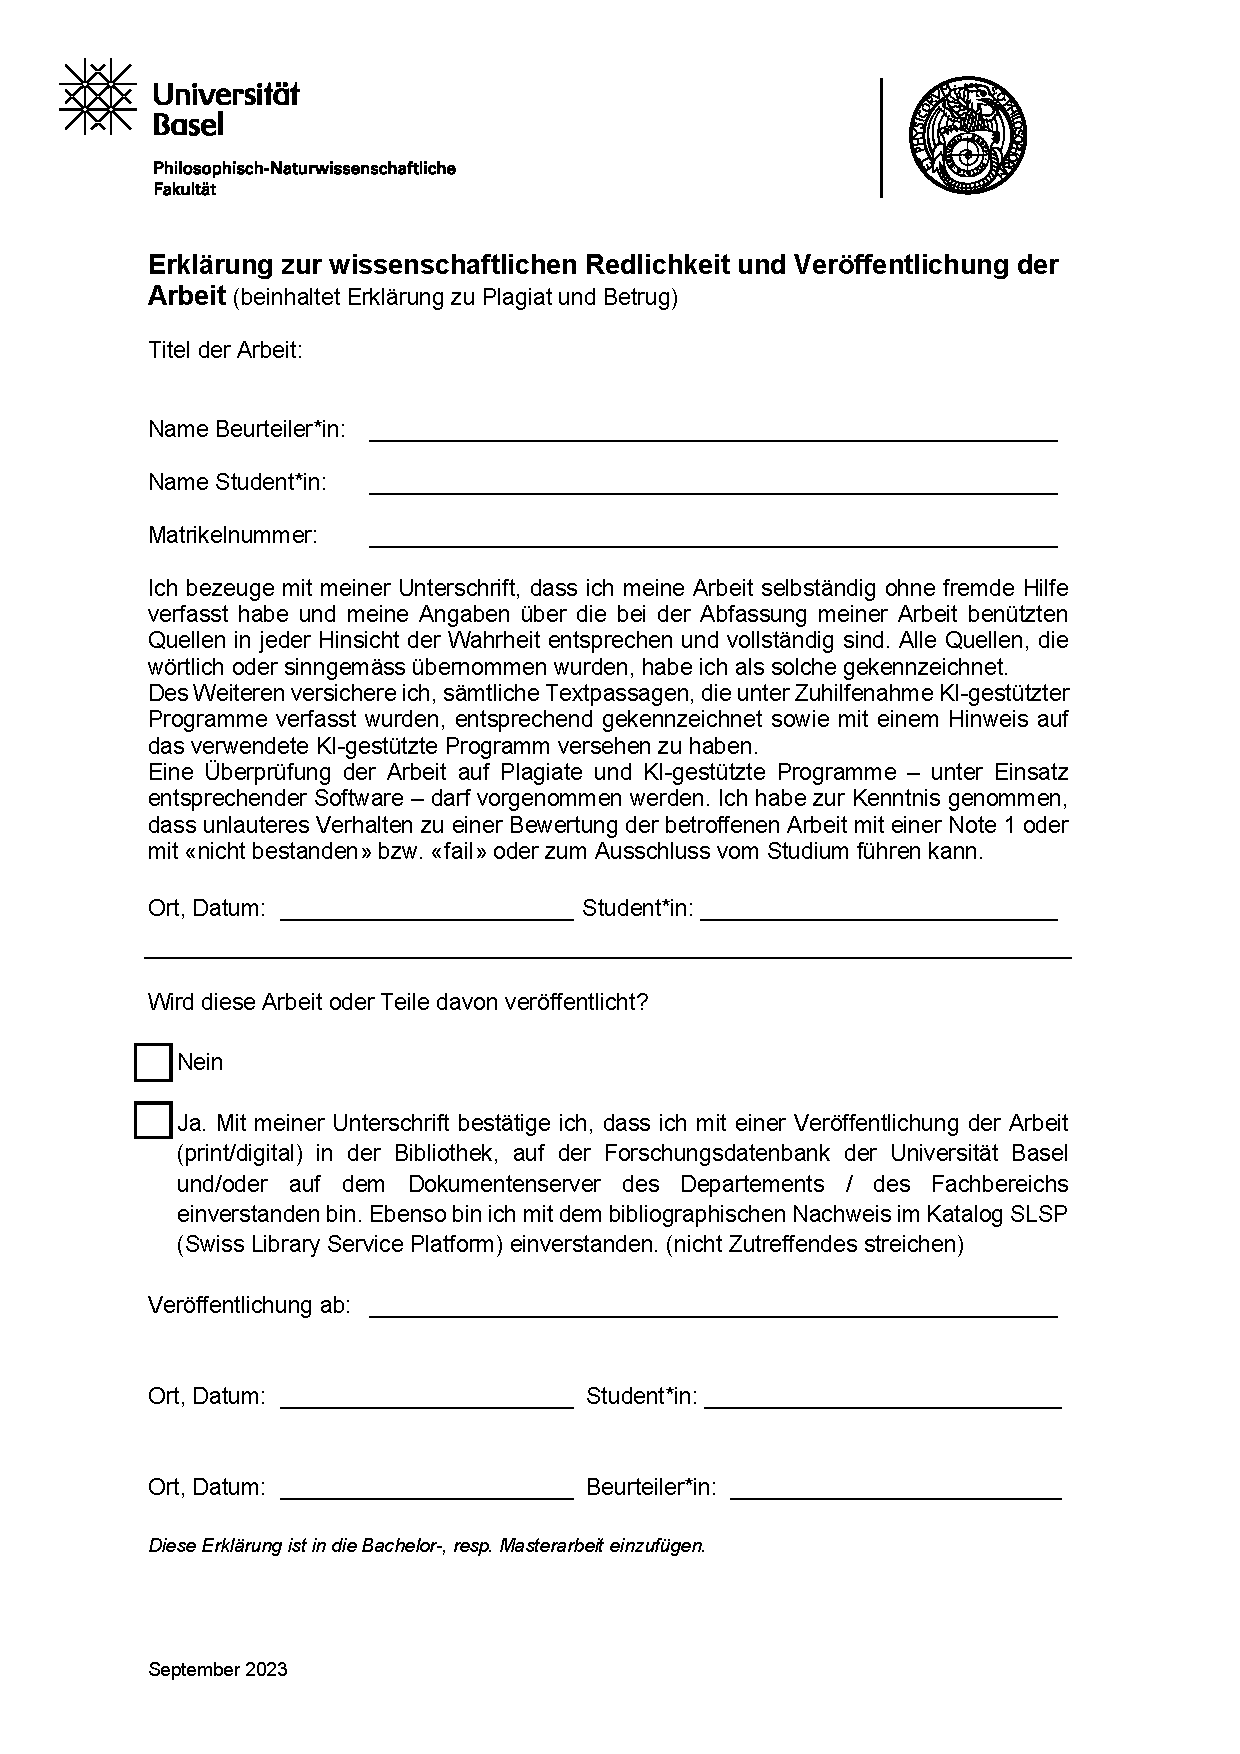
\includepdf{./Back/wissensch_Redlichkeit_D_09-2023.pdf}}
%% ----------------------------------------------------------------
\end{document}
%% ----------------------------------------------------------------
